Un environnement de travail est constitué de plusieurs fenêtres (Figure \ref{fig:spyder}) qui doivent permettre les deux modes d'utilisation. Les environnements évolués comme Spyder offrent d'autres fonctionalités\footnote{par exemple des outils de vérification (débogage).}.
\begin{itemize}
 \item Dans une fenêtre console/interpréteur, on peut écrire directement une intruction Python et l'exécuter en tapant "Entrée". 
 \item Dans la fenêtre "Editeur de texte" on peut écrire, enregistrer, ... des fichiers d'extension \verb|.py| puis les faire exécuter (bouton Executer du menu ou flèche verte(suivant les versions)) dans une fenêtre console/interpréteur)
\end{itemize}
 
 \begin{figure}[h!]
 \centering
 %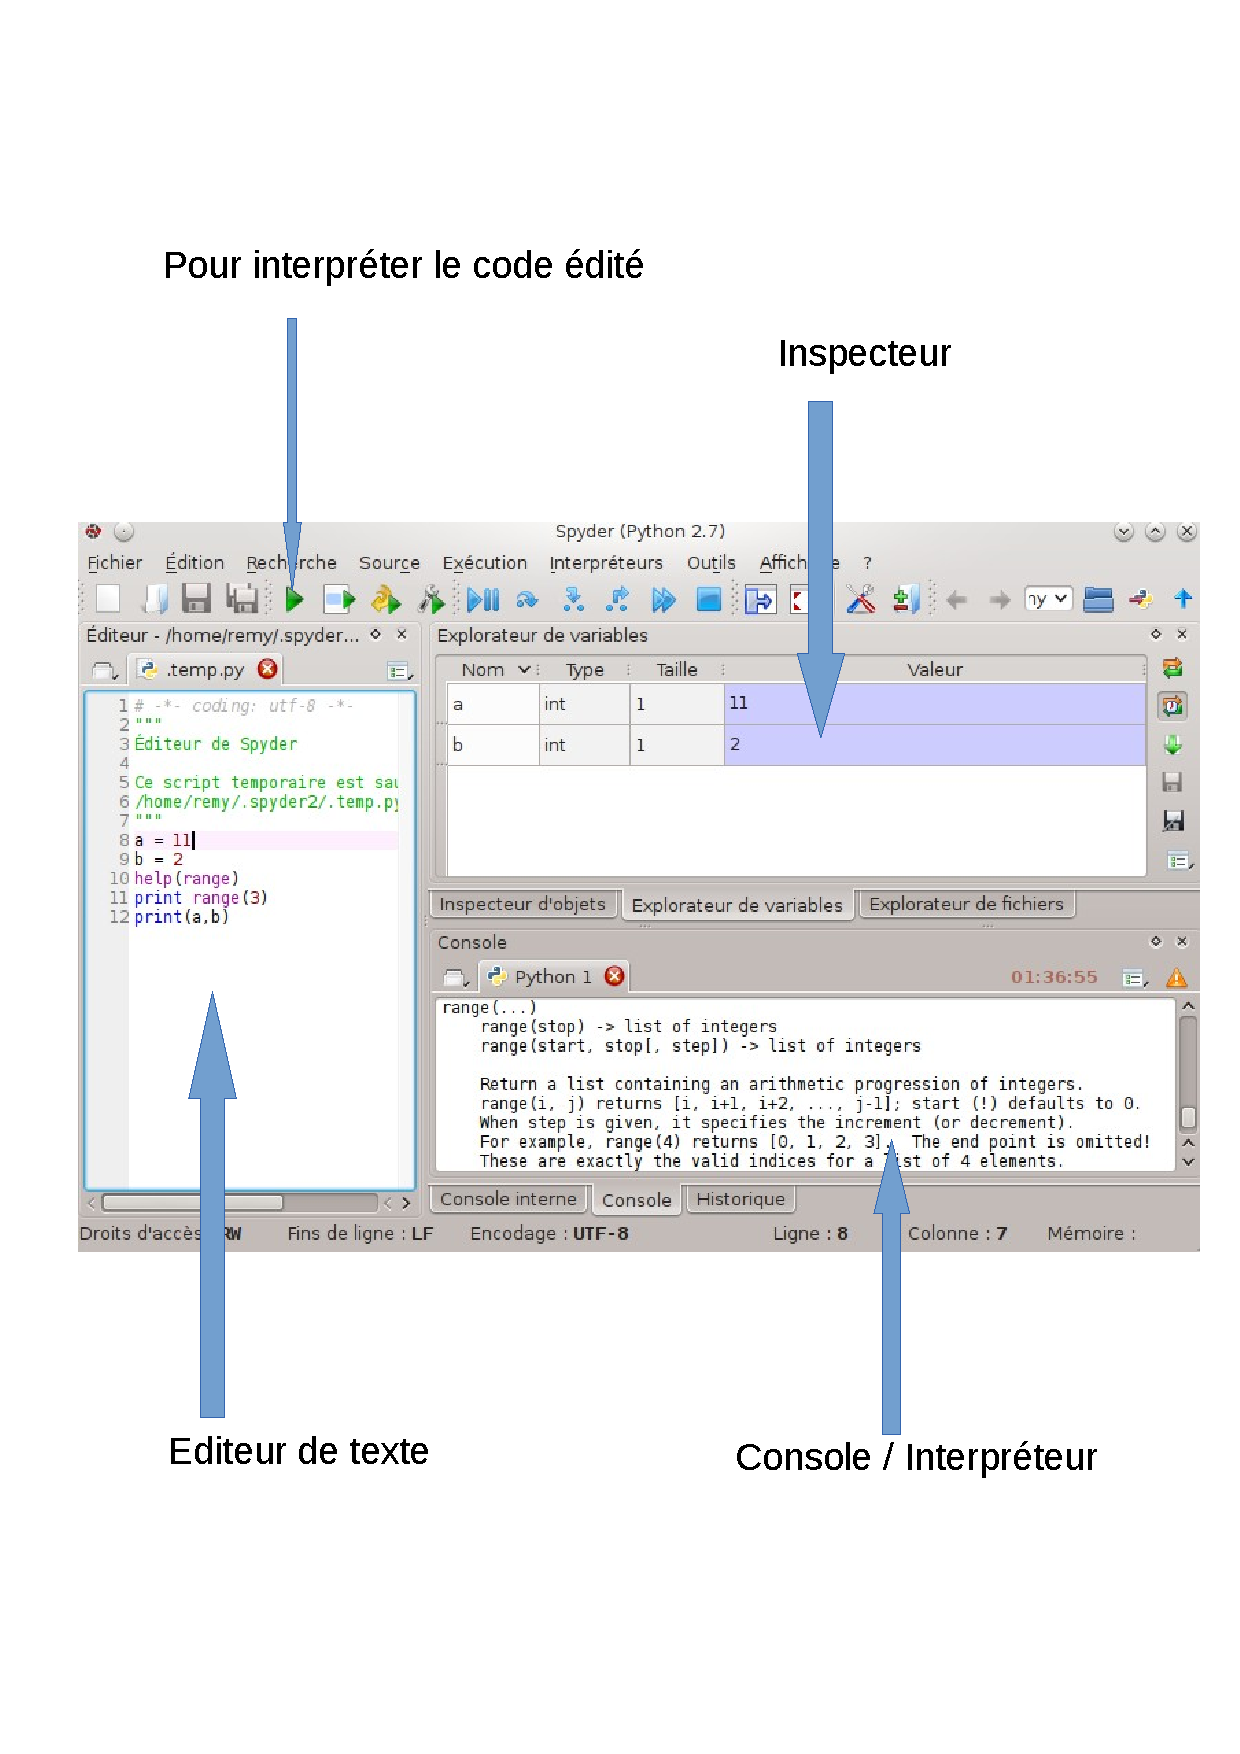
\includegraphics[width=10cm,keepaspectratio=true]{./spyder.pdf}
 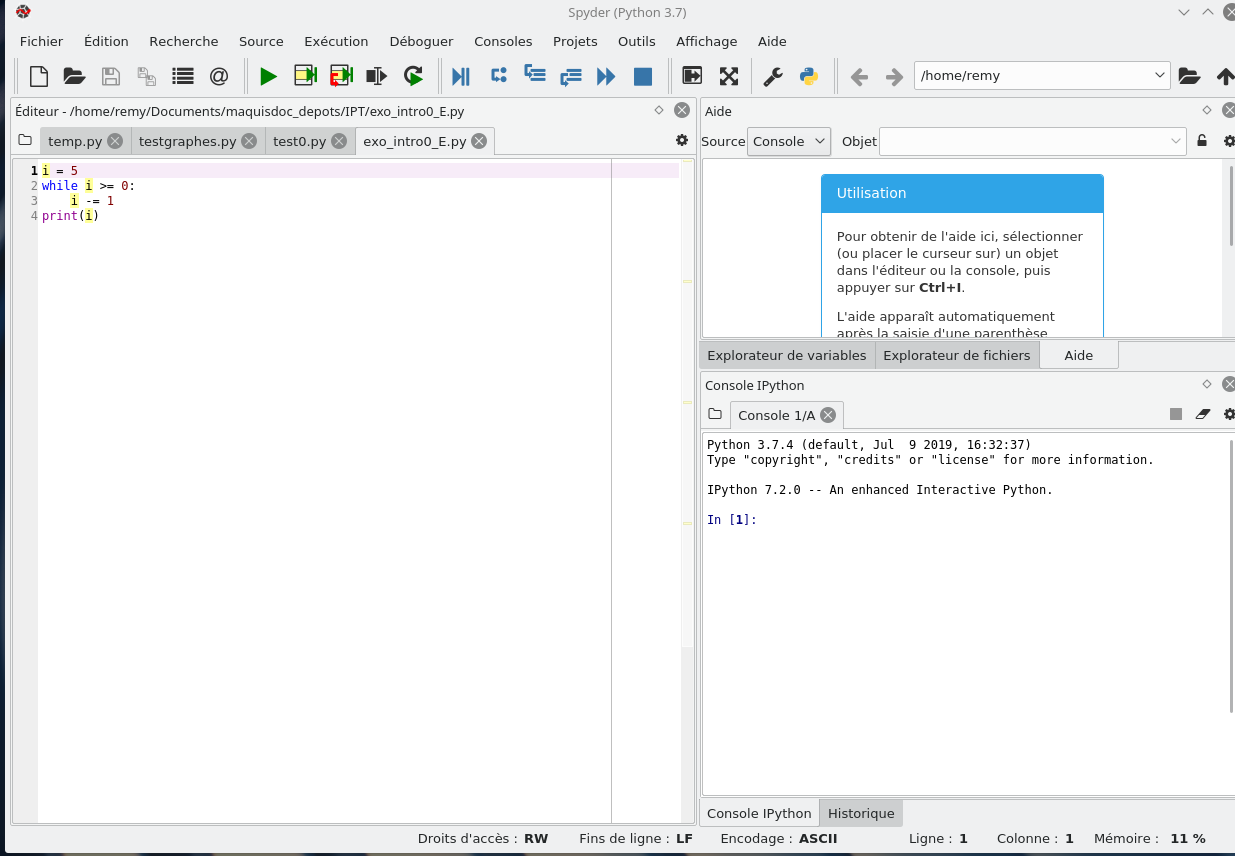
\includegraphics[width=10cm]{environnement_1.png}
 % spyder.pdf: 595x842 pixel, 72dpi, 20.99x29.70 cm, bb=0 0 595 842
 \caption{Environnement de développement spyder}
 \label{fig:spyder}
\end{figure}


Exemple avec les instructions \texttt{1+1} et \texttt{print "coucou"} ou \texttt{print("coucou")} à interpréter directement ou à exécuter par l'intermédiaire d'un fichier. Lors de l'utilisation d'un fichier, bien maitriser sa place dans l'arborescence des disques.

Il arrive souvent que le code soit mal écrit et conduise à un processus qui ne s'arrête jamais (boucle infinie). Il faut savoir comment l'arrêter.
Par exemple
 \begin{verbatim}
i = 0
while 0 < 10:
    print('coucou'+str(i))
    i+=1
 \end{verbatim}
\emph{Bien respecter l'indentation} c'est à dire les espaces en début de ligne. Interpréter dans Spyder avec la flèche verte. Repérer le petit triangle jaune avec un point d'exclamation dans le coin en haut à droite de la fenêtre de l'interpréteur.
On peut citer d'autres environnements, notamment des interpréteurs en ligne: par exemple \href{http://shell.appspot.com}{shell.appspot.com} ou \href{http://live.sympy.org/shellmobile}{live.sympy.org/shellmobile} qui est adapté aux écrans de smartphone et orienté calcul formel  (utilisant le module sympy). 
